\chapter[Resultados parciais]{Resultados Parciais}
\label{sec:resultados_parciais}

Dado o cronograma de atividades planejado para este trabalho, algumas atividades já foram realizadas. Neste capítulo apresentam-se o emprego da \textit{Revisão sistemática} e os ganhos referentes ao  \textit{Desenvolvimento prático}, com a realização da prova de conceito.

\section{Revisão sistemática} % (fold)
\label{sec:revisão_sistemática}

	A revisão bibiliográfica deste trabalho foi complementada pelo emprego da técnica de revisão sistemática. Nesta seção apresentam-se as três fases básicas da revisão sistemática definidas por \cite{Kitchenham}, \ref{sub:planejamentoRevisao} \textit{planejamento da revisão}, \ref{sub:conducaoRevisao} \textit{condução da revisão} e \ref{sub:publicacaoRevisao} \textit{reporte dos resultados da revisão}, como mostra a Figura \ref{img:processoGeralRevisao}.

	\begin{figure}[H]
			\centering
			\includegraphics[scale=0.7]{figuras/processoGeralRevisao.eps}
			\caption[Processo geral de revisão sistemática]{Processo geral de revisão sistemática, segundo \cite{Kitchenham}}
			\label{img:processoGeralRevisao}
		\end{figure}

	\subsection{Planejamento da revisão} % (fold)
	\label{sub:planejamentoRevisao}

		A revisão sistemática foi realizada entre os meses de março e junho de 2016, utilizando como fonte de busca as bases \textit{IEEE}, \textit{CAPES} e \textit{Springer}. A partir dos modelos de revisão sistemática apresentados por \cite{Kitchenham}, foi desenvolvido um protocolo de revisão, o qual possibilita, a outros pesquisadores, a repetição da pesquisa.

		\subsubsection{Objetivos e questão de pesquisa}
		
		O objetivo inicial do trabalho é estudar a problemática da auto-localização na robótica, identificando diferentes soluções em diversos contextos. Afirmado isso, foi possível realizar uma pesquisa bibliográfica com o objetivo de identificar diferentes linhas de pesquisa nesta área. Após uma análise superficial de cada linha de pesquisa, foi selecionada a linha de pesquisa que adota, como solução para a auto-localização, a utilização da técnica de SLAM, o que pode ser considerado como o marco teórico do trabalho. 

		Com a identificação do marco teórico do trabalho, a definição do foco da pesquisa torna-se uma tarefa menos árdua. Como o marco teórico deste trabalho baseia-se nas linhas de pesquisa que buscam utilizar a técnica de SLAM para realizar navegação autônoma, esta revisão sistemática teve como objetivo identificar diferentes técnicas utilizadas atualmente para solucionar o problema de SLAM em diferentes contextos, desde contextos simplificados até contextos altamente complexos.

		A definição deste objetivo da revisão dá-se pela necessidade de conhecimento amplo em relação a diferentes técnicas para solucionar o problema de SLAM. Como este trabalho buscará adaptar técnicas para um contexto simplificado, ou educacional, adicionou-se aos objetivos da revisão itens relacionados à Robótica Educacional e robôs simples.

		Segundo \cite{Kitchenham}, o primeiro passo para se realizar uma revisão sistemática é definir a sua questão de pesquisa. Desse modo, a partir da realização de uma pesquisa bibliográfica inicial, foram identificadas as seguintes questões de pesquisa: 

		\begin{itemize}
			\item \textbf{Q1}. \textit{Quais técnicas são mais utilizadas para solucionar o problema de SLAM?} e
			\item \textbf{Q2}. \textit{"Como tratar o problema de SLAM no contexto simplificado da robótica educacional?"}
		\end{itemize}

		Além das questões de pesquisa, de acordo com \cite{exemploRevisaoSistematica}, alguns outros itens devem ser detacados, como:

		\begin{itemize}
			\item \textbf{População}: comunidade acadêmica e de robótica.
			\item \textbf{Intervenção}: adaptação de técnicas para um contexto de robótica simplificado (educacional).
			\item \textbf{Controle}: utilização do \textit{Quasi-gold standard} \cite{Kitchenham}, que sera explicado mais à frente.
			\item \textbf{Resultados}: obtenção de técnicas adaptáveis ao contexto simplificado.
			\item \textbf{Aplicação}: servir de base para a implementação da segunda etapa deste trabalho de conclusão de curso, onde técnicas serão adaptadas buscando solucionar, de maneira simplificada, o problema de SLAM.

		\end{itemize} 

		A partir da definição das questões de pesquisa e dos objetivos da revisão, buscou-se definir a estratégia de pesquisa, apresentada no tópico \ref{sub:estrategias_pesquisa}.

		\subsubsection{Estratégia de pesquisa}
		\label{sub:estrategias_pesquisa}

		A estratégia de pesquisa adotada para esta revisão segue recomendações de diversos autores, como \cite{Kitchenham} e \cite{systematicReviewEngSoft}, utilizando o conceito de \textit{quasi-gold standard}.

		Segundo \cite{quasi_goldES}, \textit{gold standard} representa o conjunto completo de estudos primários referentes a uma questão de pesquisa, com máxima precisão e sensitividade. Já o \textit{quasi-gold standard}, representa um subconjunto do \textit{gold standard}, o qual vai sendo evoluído ao longo dos ciclos de busca, com o objetivo de se aproximar do \textit{gold standard}. 

		É utilizado para definir os valores de precisão e sensitividade da busca, o que possibilita a avaliação da busca realizada, verificando a necessidade de refinamento da \textit{string}, por exemplo. \cite{quasi_goldES} define precisão e sensitividade da busca da seguinte forma:

		\begin{itemize}

			\item $precisão = \frac{ERO}{EO}$ 

			\item $sensitividade = \frac{ERO}{TER}$
		\end{itemize}

		onde \textit{ERO} = número de estudos relevantes obtidos,
		
		\textit{EO} = número de estudos obtidos e

		\textit{TER} = número total de estudos relevantes.

		Esta definição possibilita a criação de critérios que avaliem a qualidade da busca, ou seja, da \textit{string} de busca utilizada. Porém, a seleção dos materiais deve seguir critérios relacionados à qualidade do material, os quais são divididos em \textit{critério de inclusão (CI)} e \textit{critério de exclusão (CE)}, como se pode observar a seguir:

		\begin{itemize}
			\item CI 1 - Os artigos devem estar escritos em inglês ou português;
			\item CI 2 - Artigos referentes à auto-localização e ao mapeamento de ambientes simultâneos (SLAM);
			\item CI 3 - Artigos com acesso gratuito, disponíveis na \textit{web} para \textit{download} ou leitura;
			\item CE 1 - Artigos que buscam solucionar o problema de auto-localização sem a utilização da técnica de SLAM, e
			\item CE 2 - Artigos que não possuem o problema de SLAM como foco principal.
		\end{itemize}

		A partir da definição da questão de pesquisa e dos objetivos da revisão, assim como a definição dos critérios de inclusão e exclusão, foi possível desenvolver uma \textit{string} de busca inicial. O idioma escolhido para a \textit{string} de busca foi o inglês, devido a sua ampla utilização nas bases de conhecimento selecionadas. Buscou-se utilizar a mesma \textit{string} de busca em todas as bases de dados pesquisadas, exceto em alguns casos em que houve a necessidade da adaptação da \textit{string} de acordo com os padrões adotados pela base.


			Com o objetivo de identificar pesquisas relacionadas à auto-localização utilizando mapeamento de ambientes simultaneamente, a \textit{string} de busca definida foi: \textit{auto-localization AND environment mapping}. Na Tabela \ref{tab:string_inicial} são apresentados os resultados obtidos a partir desta busca.

			\begin{table}[H]
			\centering
			\caption{Resultados obtidos com a \textit{string} inicial}
			\label{tab:string_inicial}
			\begin{tabular}{@{}ccc@{}}
			\hline
			\textbf{String}                                                                                    & \multicolumn{2}{c|}{\textbf{IEEE, Springer e CAPES}}                                       \\ \hline
			                                                                                                   & \begin{tabular}[c]{@{}c@{}}Nº.\\ Artigos\end{tabular} & \begin{tabular}[c]{@{}c@{}}Nº.\\ Artigos\\ relevantes\end{tabular} \\ \hline
			\textit{\begin{tabular}[c]{@{}c@{}}Auto-localization \\ AND\\ environment \\ mapping\end{tabular}} & 29                                                    & 6                                                                 \\ \hline
			\end{tabular}
			\end{table}

		Esta primeira busca foi de extrema importância para se obter uma visão inicial da pesquisa, identificando novas palavras-chave e iniciando os ciclos de busca.


		% subsection subsection_name (end)

		\subsubsection{Procedimento de seleção}

			As buscas foram realizadas com a mesma \textit{string} de busca (na maioria dos casos, como já foi explicado anteriormente) nas três bases de conhecimento científico utilizadas. A cada busca realizada, os artigos foram registrados, para que, posteriormente, os mesmos pudessem ser submetidos à avaliação da qualidade e, se comprovada a relevância do mesmo, à extração de dados.

			A seleção dos artigos deu-se a partir da leitura dos títulos, resumos e palavras-chave, classificando o artigo como relevante ou não, em um primeiro momento. Caso fosse confirmada a relevância do mesmo, o artigo passaria por uma avaliação mais profunda, a \textit{avaliação da qualidade}, como mostra o tópico \ref{sub:avaliacao_qualidade}.


		\subsubsection{Avaliação da qualidade}
		\label{sub:avaliacao_qualidade}

			A avaliação da qualidade do artigo deu-se a partir da análise do conteúdo do mesmo, focando principalmente na introdução, nos resultados e conclusões dos artigos. A avaliação positiva do artigo significa uma resposta positiva para as seguintes perguntas:

			\begin{enumerate}
				\item O estudo é interessante? (em relação aos objetivos da pesquisa)
				\item As evidências apresentadas são válidas?
				\item As evidências apresentadas são importantes?
				\item As evidências apresentadas não contradizem autor algum selecionado como pilar da pesquisa?
			\end{enumerate}

			Com a confirmação da qualidade do material, o mesmo foi exposto à extração de dados, ou seja, à leitura completa e detalhada do artigo.

		\subsubsection{Extração de dados}

			Com o objetivo de organizar os dados obtidos, facilitando o manuseio das informações, os dados extraídos de cada artigo foram registrados conforme o modelo apresentado na Tabela \ref{tab:padrao_dados_extraidos}.

			\begin{table}[H]
				\centering
				\caption{Exemplo de registro de material}
				\label{tab:padrao_dados_extraidos}
				\begin{tabular}{@{}ccccc@{}}
					\hline
					\textbf{Título} & \textbf{Autor(es)} & \textbf{\begin{tabular}[c]{@{}c@{}}Data de\\ publicação\end{tabular}} & \textbf{\begin{tabular}[c]{@{}c@{}}Fonte da\\ publicação\end{tabular}} & \textbf{\begin{tabular}[c]{@{}c@{}}Listagem das\\ informações\\ importantes\end{tabular}} \\ \hline
					\textit{\begin{tabular}[c]{@{}c@{}}Integration of Vision\\ based SLAM and \\ Nonlinear Filter for\\ Simple Mobile Robot\\ Navigation\end{tabular}} & \begin{tabular}[c]{@{}c@{}}Dae Hee Won,\\ Young Jae Lee,\\ Sangkyung Sung,\\ Taesam Kang\end{tabular} & 2008                                                                  & IEEE                                                                   & \begin{tabular}[c]{@{}l@{}}-Utilização de\\ sensor de visão\\ e encoders.\\ -Filtro de \\ partículas\end{tabular}                      \\ \hline
				\end{tabular}
			\end{table}

		
	% subsection planejamento_da_revisão (end)

	\subsection{Condução da revisão} % (fold)
	\label{sub:conducaoRevisao}
		
		Durante a condução da revisão, a busca efetiva dos materiais é realizada, os ciclos de busca são documentados e a \textit{string} de busca é refinada, como afirma \cite{estudoPrimarioSecundario}.

		Esta pesquisa foi realizada entre os meses de março e junho de 2016. A \textit{string} de busca apresentada no tópico \ref{sub:estrategias_pesquisa} resultou em uma visão considerada fraca, pelo pesquisador e seus orientadores, sobre a auto-localização e o mapeamento de ambientes, peças chave da técnica de SLAM. Além disso, essa busca possibilitou a criação do \textit{quasi-gold standard} inicial, com apenas um artigo: \textit{Auto-localização e construção de de mapas de ambiente para robôs móveis baseados em visão omnidirecional estéreo} \cite{localizacaoEMapeamentoPaulo}. 

		Desse modo, foi necessária a realização de uma pesquisa manual para obter maior conhecimento sobre o tema e as palavras-chave a serem usadas para garantir maior qualidade dos resultados obtidos. Com a realização desta pesquisa, os seguintes artigos foram adicionados ao \textit{quasi-gold standard}:

		\begin{itemize}
			\item \textit{The Cleaning Robot Project: Aplicação do Filtro de Kalman na Auto-Localização de um Sistema Robótico Autônomo} \cite{theCleaningProject},
			\item \textit{Integration of Vision based SLAM and Nonlinear Filter for Simple Mobile Robot Navigation} \cite{integrationVisionSLAMnonlinear} e
			\item \textit{A Solution to the Simultaneous Localization and Map Building (SLAM) Problem} \cite{slamProblem}.
		\end{itemize}

		A partir da análise destes artigos inciais, foi possível identificar diversas palavras-chave que levavam à pesquisa desejada, possibilitando refinamento da \textit{string} de busca. Adicionando à mesma novos termos, como \textit{"SLAM problem"} e \textit{"simultaneous"}, evoluindo a \textit{string} e obtendo o seguinte resultado: \textit{"simultaneous AND auto-localization AND environment mapping AND SLAM problem"}.
		
		O ciclo de busca utilizando esta \textit{string} gerou poucos resultados, selecionando apenas um para análise: \textit{Improved global localization of an indoor mobile robot via fuzzy extended information filtering} \cite{ROB:1764504}. Com o objetivo ampliar a abrangência da busca, optou-se por modificar a palavra-chave \textit{auto-localization} por apenas \textit{localization}, obtendo a seguinte \textit{string} de busca: \textit{"simultaneous AND localization AND environment mapping AND SLAM problem"}.

		Com a realização deste novo ciclo de busca, diversos artigos relevantes foram identificados e adicionados ao \textit{quasi-gold standard}. Os artigos presentes no \textit{quasi-gold} corrente foram encontrados com esta nova busca, evidenciando uma certa qualidade da \textit{string} de busca. Os artigos adicionados ao \textit{quasi-gold standard} durante este ciclo são:

		\begin{itemize}
			\item \textit{A Simultaneous Localization and Mapping Algorithm in Complex Environments: SLASEM} \cite{slasem},
			\item \textit{A Neuro-Fuzzy Assisted Extended Kalman Filter-Based Approach for Simultaneous Localization  and  Mapping (SLAM) Problems} \cite{neurofuzzi},
			\item \textit{Map Management for Efficient Simultaneous Localization and Mapping (SLAM)} \cite{mapManagement} e
			\item \textit{Simultaneous Localization and Map Building by Integrating a Cache of Features} \cite{integratingCacheFeat}.
		\end{itemize}

		Com o intuito de especificar mais a busca, foi adicionada, devido a uma dica do orientador prof. Dr. Maurício Serrano, a palavra-chave \textit{"simple robots"} à \textit{string} de busca, chegando a seguinte \textit{string}: \textit{"simultaneous AND localization AND environment mapping AND SLAM problem OR ("simple mobile robots" AND slam)"}.

		Com esta mudança, obteve-se outra visão desta pesquisa como um todo. Dessa forma, foram identificadas diversas pesquisas que buscam solucionar problemas de locomoção, como o problema de SLAM, em contextos limitados, da mesma forma que objetivo geral deste trabalho. Por fim, foram adicionados ao \textit{quasi-gold standard}, os seguintes artigos:

		\begin{itemize}
			\item \textit{BatSLAM: Simultaneous Localization and Mapping Using Biomimetic Sonar} \cite{batslam},
			\item \textit{Neural Network-Based Multiple Robot Simultaneous Localization and Mapping} \cite{neuralNetwork} e
			\item \textit{Visual simultaneous localization and mapping: a survey} \cite{surveyLocalization}.
		\end{itemize}

		Como é possível observar, os artigos selecionados para adição no \textit{quasi-gold standard} não envolviam temas referentes a robôs simples, apesar da afirmação de que esta mudança havia modificado a visão da pesquisa. Artigos referentes a este tema não foram adicionados ao \textit{quasi-gold standard} devido ao fato dos mesmos serem \textit{barrados} pelo critério de exclusão \textit{"CE 2 - Artigos que não possuam o problema de SLAM como foco principal"}. 

		Em contrapartida, este ciclo possibilitou o conhecimento de novos termos, viabilizando um refinamento eficiente para o próximo ciclo de busca.

		No próximo ciclo de busca, foram adicionadas palavras-chave referentes à Robótica Educacional e às estratégias de resolução do problema de SLAM, como mostra a \textit{string}: \textit{"(Simple mobile robot? AND (SLAM OR auto-localization)) AND (map* OR education* robot*) AND strateg*"}. Além de adicionar estes novos termos, utilizou-se de técnicas disponíveis nas bases, como a utilização de \textit{'?'}, que representa qualquer caractere, e \textit{'*'}, que significa que quaisquer caracteres precedidos dos caracteres anteriores ao \textit{'*'} serão considerados.

		Para realização desta busca, foi necessária a adaptação da \textit{string} de busca durante a pesquisa na base de dados \textit{Springer}, devido a diferenças nos padrões de definição da \textit{string}. Para esta adaptação, novas palavras-chave precisaram ser selecionadas, as quais foram obtidas a partir dos resultados advindos das outras bases, com a mesma \textit{string}.

		A \textit{string} adaptada para a base \textit{Springer} foi: \textit{"(Simple AND mobile AND robot AND SLAM AND localization AND mapping) AND (educational AND navigation AND simultaneous) AND strategies"}.

		Ao realizar esta busca, foi observado que os resultados atendiam, em sua maioria, ao desejado pela pesquisa, sendo muitos artigos selecionados para análise e avaliação e alguns adicionados ao \textit{quasi-gold standard}, como:

			\begin{itemize}
				\item \textit{Incremental SLAM with Backtracking Data Association for Mobile Robots} \cite{incrementalSLAM},
				\item \textit{Mapping and Pursuit-Evasion Strategies For a Simple Wall-Following Robot} \cite{wall_following} e
				\item \textit{A Simple and Parallel Algorithm for Real-Time Robot Localization by Fusing Monocular Vision and Odometry/AHRS Sensors} \cite{fusingSensorsParallel}.
			\end{itemize}

		Com a realização desta busca, foram obtidos 27 artigos, restando apenas 20 após a avaliação da relevância dos mesmos para a pesquisa. Desde o primeiro ciclo de busca, diversos artigos foram considerados relevantes para a pesquisa, chegando a um número de 42 (quarenta e dois) artigos relevantes.
		
		Ou seja, aplicando os conceitos de \textit{precisão} e \textit{sensitividade}, temos que:

		\begin{itemize}
			\item $sensitividade = \frac{20}{42}$ 
			\item $precisao = \frac{20}{27}$
		\end{itemize}

		Desse modo, foi obtida uma \textit{sensitividade} de 47\% e uma precisão de 74\%, dando fim aos ciclos de busca com 42 artigos selecionados e analisados. A Tabela \ref{tab:string_final} apresenta, de maneira resumida, a evolução da \textit{string} de busca, comparando a \textit{string} inicial com a \textit{string} final da pesquisa.

\begin{table}[H]
\centering
\caption{Comparação das \textit{strings} inicial e final}
\label{tab:string_final}
\begin{tabular}{@{}c|c|c|c|c@{}}

\multirow{2}{*}{\textbf{String}} & \multirow{2}{*}{\textbf{\begin{tabular}[c]{@{}c@{}}Fonte de \\ busca\end{tabular}}} & \multicolumn{2}{c|}{\textbf{Resultados}} & \multirow{2}{*}{\textbf{Observações}}                                                                                                                                                        \\ \cline{3-4}
                                 &                                                                                     & \textbf{Total}   & \textbf{Relevantes}   &                                                                                                                                                                                              \\ \hline
\multirow{3}{*}{Inicial}         & \textit{IEEEXplore}                                                                 & 2                & 1                     & \multirow{3}{*}{\begin{tabular}[c]{@{}c@{}}String construída sem o conhecimento\\ necessário para utilização das palavras-\\ chave que representam a pesquisa.\end{tabular}}                 \\ \cline{2-4}
                                 & \textit{Springer}                                                                   & 19               & 2                     &                                                                                                                                                                                              \\ \cline{2-4}
                                 & \textit{CAPES}                                                                      & 8                & 3                     &                                                                                                                                                                                              \\ \hline
\multirow{3}{*}{Refinada}        & \textit{IEEEXplore}                                                                 & 17               & 13                    & \multirow{3}{*}{\begin{tabular}[c]{@{}c@{}}String refinada, ao longo de diversos ciclos de \\ busca, adicionando novas palavras-chave e\\ obtendo resultados mais específicos.\end{tabular}} \\ \cline{2-4}
                                 & \textit{Springer}                                                                   & 6                & 3                     &                                                                                                                                                                                              \\ \cline{2-4}
                                 & \textit{CAPES}                                                                      & 4                & 4                     &                                                                                                                                                                                              \\ \hline
\end{tabular}
\end{table}

Durante a realização de cada ciclo, os artigos foram analisados, avaliados e seus dados foram extraídos como fonte de estudo para a realização deste trabalho de conclusão de curso. Na seção \ref{sub:publicacaoRevisao}, serão apresentados os resultados de maneira organizada e simplificada.

		% subsection condução_da_revisão (end)

	\subsection{Publicação dos resultados} % (fold)
	\label{sub:publicacaoRevisao}
		
		A primeira etapa deste trabalho de conclusão de curso pode ser vista como o resultado geral desta revisão sistemática, onde conceitos, termos, abordagens e qualquer informação utilizada no trabalho é fruto, seja direta ou indiretamente, desta revisão sistemática.

		Com o objetivo de documentar os resultados diretos desta revisão sistemática, estes foram registrados como as técnicas utilizadas atualmente para solucionar o problema de SLAM em diferentes contextos. 

		Com a realização desta revisão, foi possível identificar \textit{áreas} mutáveis nas diferentes soluções do problema de SLAM. As áreas identificadas são \textit{"arquitetura da solução"} \ref{sub:arquitetura_solucao}, \textit{"técnica probabilística utilizada"} \ref{sub:prob_usada} e \textit{"informações disponíveis"} \ref{sub:infos_disponiveis}. Em cada solução, os autores buscaram se adequar ao contexto trabalhado, seja a partir da disponibilidade de sensores específicos ou da capacidade computacional disponível.


		\subsubsection{Arquitetura da solução}
		\label{sub:arquitetura_solucao}

			A arquitetura da solução, na grande maioria dos estudos, foi definida a partir do requisito computacional. Ou seja, a limitação computacional presente nos robôs simples levou os autores a buscarem arquiteturas que contornassem esse problema, como mostra \cite{redeComunicacaoIndustria}. Entre as diversas arquiteturas, as mais comumente utilizadas são as que buscam processar as informações em um computador, utilizando o robô apenas para obtenção das informações, como ilustra a Figura \ref{img:arquitetura_mais_utilizada}.

			\begin{figure}[H]
				\centering
				\includegraphics[scale=0.9]{figuras/arquitetura_mais_utilizada.eps}
				\caption[Arquitetura de comunicação]{Arquitetura de comunicação}
				\label{img:arquitetura_mais_utilizada}
			\end{figure}

			De acordo com a Figura \ref{img:arquitetura_mais_utilizada}, o robô será responsável apenas por obter informações do ambiente, ou seja, recuperar os dados obtidos a partir dos sensores disponíveis. O computador, em posse das informações sobre o ambiente, ou seja, os pontos de referência, a quantidade de rotações em cada roda, a distância e cores de objetos, por exemplo, será responsável por processar toda a informação, construindo um mapa lógico para possibilitar a localização do robô em relação ao ambiente, como apresenta \cite{redeComunicacaoIndustria}.

			Geralmente, são utilizados dois mapas simultâneos, um presente no robô (local) e outro, mais completo, presente no computador (remoto). O mapa local é, basicamente, um vetor de pontos \textit{'p'} em relação a um tempo \textit{'t'}, como explica \cite{circumventingAssociationSLAM}. O computador utiliza este mapa local, que é disponibilizado pelo robô, para completar, corrigir e atualizar o mapa remoto, mesclando informações e utilizando, geralmente, filtros probabilísticos para maximizar sua precisão \cite{localizacaoEMapeamentoPaulo}.

			As decisões referentes à navegação são geradas a partir da análise do mapa remoto, já que o mapa local é incompleto e inconsistente, como afirma \cite{redeComunicacaoIndustria}. A utilização desta arquitetura de mapeamento remoto e local torna prática a realização de navegações com múltiplos robôs, como apresenta, \cite{redeComunicacaoIndustria}, em seu trabalho sobre rede de comunicação sem fio para navegação de múltiplos robôs. 

			Seguindo esta arquitetura, \cite{neuralNetwork} e \cite{multiRobots} também desenvolveram sistemas de resolução do problema de SLAM com a utilização de múltiplos robôs, mostrando a viabilidade da sua utilização. Neste tipo de trabalho, os robôs colaboram entre si, pois, como a informação obtida é centralizada em um computador único, as decisões referentes à navegação de um determinado robô são resultados do processamento das informações obtidas por todos os robôs, maximizando a vizão global de cada robô \cite{redeComunicacaoIndustria}.

			De qualquer forma, independente da arquitetura da solução utilizada, os erros advindos dos sensores sempre serão um problema sério a ser resolvido \cite{circumventingAssociationSLAM}. Com o objetivo de solucionar este problema, a comunidade de robótica vê-se presa à utilização de estruturas matemáticas probabilísticas, como afirma \cite{circumventingAssociationSLAM}. As seções \ref{sub:kalman}, \ref{sub:filtro_de_partículas} e \ref{sub:prob_usada} apresentam as estruturas probabilísticas mais utilizadas atualmente, assim como suas vantagens e desvantagens.

		\subsubsection{Técnica probabilistica utilizada}
		\label{sub:prob_usada}

			Para a realização de uma navegação específica, primeiramente, o robô deverá obter informações sobre o ambiente \cite{roboticaIndustrial}. Para isso, é necessária a utilização de sensores que captem estas informações, seja a partir de odometria, infra-vermelho ou vídeo. Entretanto, estes sensores são munidos de uma margem de erro que, muitas vezes, prejudica a navegação e a auto-localização como um todo \cite{interacaoRoboAmbiente}. De acordo com \cite{circumventingAssociationSLAM}:

			\begin{quote}
				\textit{Devido à natureza imperfeita dos sensores, à falta da previsibilidade em ambientes reais e à necessidade de aproximações para alcançar decisões computacionais, a robótica é uma ciência que depende de algorítmos probabilisticos}.
			\end{quote}

			Desse modo, a comunidade de robótica vem buscando, na matemática, soluções probabilísticas que minimizem esta margem de erro, como afirma \cite{surveyLocalization}. Entre as soluções mais utilizadas, encontram-se, no topo da lista, os filtros de \textit{Kalman} e \textit{partículas}, como pode ser observado nas seções \ref{sub:kalman} e \ref{sub:filtro_de_partículas}, respectivamente.

			Alguns autores, como, por exemplo, \cite{comparacaoKalmanParticulas}, vêm estudando as duas técnicas e comparando-as com o intúito de selecionar a \textit{"melhor"} técnica. Entretando, o termo \textit{"melhor"} é relativo, neste caso, a depender do contexto em que será aplicado o filtro probabilístico, como afirma \cite{comparacaoKalmanParticulas}.

			O estudo de \cite{comparacaoKalmanParticulas} exemplifica, com clareza, as comparações entre os filtros de partícula e de Kalman, ao utilizar as duas técnicas para solucionar o problema de SLAM com um robô móvel munido de sensores a laser. De acordo com a relatividade do termo \textit{"melhor"}, nesta ocasião, o autor buscou apresentar apenas algumas vantagens e desvantagens dos dois filtros, como pode-se observar nas seções \ref{sub:kalman} e \ref{sub:filtro_de_partículas}. 

		\subsubsection{Informações disponíveis}
		\label{sub:infos_disponiveis}

			Na robótica móvel, existem diversas maneiras de se obter informações sobre o ambiente, a partir da utilização de sensores específicos para informações específicas \cite{interacaoRoboAmbiente}. Entre os sensores mais utilizados, encontram-se os \textit{sonares, sensores infra-vermelho, câmeras de vídeo, sensores de distância, sensores RGB e sensores odométricos}. A partir do ambiente em que se deseja navegar, faz-se necessária a seleção dos sensores adequados para o mesmo.

			Além do tipo de sensor escolhido, deve-se levar em consideração algumas características do mesmo, como o alcance, desempenho e precisão, por exemplo. Conhecer a margem de erro dos sensores é essencial, como afirma \cite{wall_following}. 

			Como foi explicado no tópico \ref{sub:prob_usada}, os sensores possuem margens de erro que podem prejudicar a navegação e a auto-localização do robô. Em busca de tentar solucionar este problema, além da utilização de filtros probabilísticos, diversos autores buscam utilizar múltiplos sensores, integrando as informações dos mesmos para minimizar a margem de erro na informação, como mostram \cite{fusingSensorsParallel}, \cite{neuralNetwork} e \cite{slamProblem}. 

			De acordo com \cite{agenteExploratorioKalman}, há três tipos de integração entre sensores: \textit{complementar}, onde os sensores têm apenas uma visão parcial do ambiente, unindo as informações para obter uma visão mais completa; \textit{competitiva}, onde dois ou mais sensores competem para obter a informação com maior precisão, como a medição da distância de um único objeto utilizando sonar e sensor a laser, por exemplo; e \textit{cooperativa}, quando os sensores cooperam entre si para obter informações que não seriam possíveis com a utilização de apenas um, como a geração de informações em três dimensões, por exemplo.

			Entre os sensores citados anteriormente, o sensor odométrico, geralmente, é utilizado em qualquer sistema de navegação sobre eixos, de acordo com \cite{explore_marte}. Este sensor recupera os dados sobre rotações realizadas nas rodas em que o mesmo se encontra, possibilitando a mensuração da distância percorrida, assim como a identificação de curvas, por exemplo \cite{ROB:1764504}. 

			Entretanto, como afirma \cite{iterated_Dslam}, sensores odométricos geram erros acumulativos, ou seja, quanto maior for a navegação, maior será o erro total do sensor. Trabalhar com sensores assim gera uma certa dificuldade. Entretanto, com a utilização de filtros probabilísticos, como apresentado na seção \ref{sub:prob_usada}, este erro pode ser reduzido, viabilizando sua utilização.

			Já a utilização de câmeras de vídeo, segundo \cite{agenteExploratorioKalman}, além de necessitar de \textit{landmarks} verificáveis através do processamento de imagens, as mesmas exigem requisitos computacionais que, muitas vezes, acabam por inviabilizar sua utilização.

			O sensor ultrasônico, que será utilizado durante a segunda etapa deste trabalho, diferentemente das câmeras de vídeo, são simples, rápidos e baratos, de acordo com \cite{agenteExploratorioKalman}. Entretanto, sua utilização acaba por limitar o contexto de navegação, devido ao seu limite de alcance. Ou seja, em um ambiente aberto, o sensor ultrasônico não será capaz de identificar obstáculo algum. Além da sua limitação de alcance, \cite{agenteExploratorioKalman} apresenta algumas características que podem problematizar sua utilização:

			\begin{enumerate}
				\item \textit{pobre direcionalidade}: não são capazes de identificar a direção do obstáculo identificado, apenas sua distância;
				\item \textit{passíveis de ruídos}: ruídos são comuns durante a utilização de sonares, seja devido a interferências de outros sensores, ou a partir da sua margem de erro padrão, por exemplo.
				\item \textit{reflexão especular}: O sensor emite o sinal sonoro em formato de cone, possibilitando a obtenção de erros relacionados à angulação de incidência. 
			\end{enumerate}

			Com foi definido por \cite{agenteExploratorioKalman}, umas das características importantes da utilização do sonar é a reflexão especular, devido a sua emissão em formato de cone, como é apresentado de forma clara na Figura \ref{img:cone}.

			\begin{figure}[H]
				\centering
				\includegraphics[scale=0.5]{figuras/cone.eps}
				\caption[Emissão do sinal sonoro - sonar]{Emissão do sinal sonoro - sonar}
				\label{img:cone}
			\end{figure}

			Outro detalhe importante a ser analisado, segundo \cite{agenteExploratorioKalman}, é a velocidade de emissão do sinal. Esta deve ser relacionada a necessidade de obtenção das informações, ou seja, dependendo da velocidade de navegação atual do robô, a velocidade de emissão deve ser atualizada. Desse modo, se o robô se movimenta rapidamente, devem ser gerados sinais a uma frequência alta, possibilitando a reação do robô a eventos inesperados \cite{agenteExploratorioKalman}.

			Com a emissão de sinais sonoros enquanto o robô se movimenta, como foi sugerido anteriormente, deve-se levar em consideração o atraso no mapeamento, já que, ao obter o retorno do sinal, o robô já não se encontra no mesmo local \cite{agenteExploratorioKalman}, inserindo erros na navegação, o que pode prejudicá-la. 

			Outro problema bastante recorrente com a utilização de sonares é a identificação de cantos em paredes, por exemplo. Como a emissão do sinal é feita no formato de cone, quando a extremidade do cone alcança a parede, a mesma é refletida fornecendo a informação ao robô. O mesmo acontece do outro lado do cone, deixando o centro invisível ao sinal sonoro. O impacto deste problema é proporcional a distância entre o robô e o objeto, como já foi explicado ao longo do trabalho.

	% subsection publicação_dos_resultados (end)

	A Tabela \ref{tab:resultadosRevisao} apresenta de maneira organizada a contabilização dos resultados da revisão, de acordo com as áreas destacadas anteriormente. Encontram-se nesta Tabela apenas os artigos que solucionaram, de alguma maneira, o problema de SLAM.

\begin{table}[H]
\centering
\caption{Contabilização de estratégias (SLAM)}
\label{tab:resultadosRevisao}

\begin{tabular}{@{}cccc@{}}
\hline
\textbf{\begin{tabular}[c]{@{}c@{}}Arquitetura\\ de processamento\end{tabular}}                    & \textbf{Filtro} & \textit{\textbf{Inputs}}                                                                                                                         & \textbf{\begin{tabular}[c]{@{}c@{}}Nº.\\ Artigos\end{tabular}} \\ \hline
                                                                                                   & Kalman          & \begin{tabular}[c]{@{}c@{}}laser, vídeo, odometria,\\ sonar, infra-vermelho,\\ câmera términa, \\ kinect RGB, \\ sonar biomimético.\end{tabular} & 12                                                             \\ \cline{2-4} 
\multirow{-2}{*}{\begin{tabular}[c]{@{}c@{}}Processamento\\ remoto\end{tabular}}                   & Partículas      & \begin{tabular}[c]{@{}c@{}}Câmera de vídeo,odometria, \\ laser, sonar,magnetômetro, \\ sensor de rádio.\end{tabular}                             & 5                                                              \\ \hline
                                                                                                   & Kalman          & \begin{tabular}[c]{@{}c@{}}sensor de distância (laser),\\ odometria, identificador de\\ landmarks (simulado) e sonar.\end{tabular}               & 3                                                              \\ \cline{2-4} 
\multirow{-2}{*}{\begin{tabular}[c]{@{}c@{}}Processamento\\ local\end{tabular}}                    & Partículas      & Sonar e odometria                                                                                                                                & 1                                                              \\ \hline
                                                                                                   & Kalman          & \begin{tabular}[c]{@{}c@{}}laser (range),\\ vídeo e\\ odometria\end{tabular}                                                                     & 3                                                              \\ \cline{2-4} 
\multirow{-2}{*}{\begin{tabular}[c]{@{}c@{}}Processamento\\ remoto + múltiplos robôs\end{tabular}} & Partículas      & 0                                                                                                                                                & 0                                                              \\ \hline
\rowcolor[HTML]{C0C0C0} 
\multicolumn{3}{|c|}{\cellcolor[HTML]{C0C0C0}\textbf{Total}}                                                                                                                                                                                                            & 24                                                             \\ \hline
\end{tabular}
\end{table}


	%CAPES:
		%Planning exploration strategies for simultaneous localization and mapping
			%Arquitetura: processamento remoto + multiplos robos
			%Filtro: Algoritmo dele baseado em kalman
			%input: video (imagens) e odometria
		%Módulo de Auto-localização para um agente exploratório usando filtro de kalman
			%Arquitetura: processamento remoto
			%Filtro: Kalman
			%input: 8 sensores infra-vermelho e odometria
		%Autonomous Multisensor Calibration and Closed-loop fusion for SLAM
			%Arquitetura: Processamento remoto
			%Filtro: Kalman
			%input: camera de vídeo, sonar, odometria, SICK laser (sonar 360º), kinect RGB, sensor a laser e câmera térmica
		%BatSLAM: Simultaneous Localization and Mapping Using Biomimetic Sonar
			%Arquitetura: processamento remoto
			%filtro: partículas
			%input: sonar biomimético (criaram um sonar que imita o sonar dos morcegos)
		%Melhoramento do Desempenho do Robot de Serviço de Limpeza
			%Arquitetura: processamento remoto
			%filtro: Kalman e partícula (comparando)
			%input: câmera de vídeo, sonar e odometria
		%GPU based real-time SLAM of six-legged robot
			%Arquitetura: processamento remoto
			%filtro: adaptação Kalman
			%input: Vídeo e odometria
		%A Robust Regression Model for Simultaneous Localization and Mapping in Autonomous Mobile Robot
			%Arquitetura: processamento remoto
			%filtro: Kalman
			%input: sensor de distância (laser) e odometria 
		%The Cleaning Robot Project Aplicação do Filtro de Kalman na Auto-Localização de um Sistema Robótico Autónomo
			%Arquitetura: processamento remoto
			%filtro: Kalman
			%input: câmera de vídeo, sonar, sharps (parecido com sonar, mas direcionado e mais precisos) e odometria
		%Absolute localization for a mobile robot using place cells
			%Arquitetura: processamento remoto
			%filtro: Kalman
			%input: Sonar, vídeo e odometria
		%Integration of Vision based SLAM and Nonlinear Filter for Simple Mobile Robot Navigation
			%Arquitetura: processamento remoto
			%filtro: partículas
			%input: vídeo e odometria

		%10 ARTIGOS NA CAPES - de aplicação de SLAM (tirando os outros)
	%------------------------------------------------------------------
	%IEEE:
		%Unmanned Autonomous Vehicle Control & SLAM Problem in 2-D environment
			%Arquitetura: processamento remoto
			%Filtro: kalman
			%input: sensor de distância (laser) e odometria
		%Set-Membership Approach to the Kidnapped Robot Problem
			%Arquitetura: processamento remoto
			%Filtro: partículas
			%input: sonar, odometria
		%Simultaneous Localization and Map Building by Integrating a Cache of Features
			%Arquitetura: processamento remoto
			%Filtro: Kalman
			%Input: sensor distância - laser
		%Simultaneous Localization and Mapping: A Pseudolinear Kalman Filter (PLKF) Approach
			%Arquitetura: não disse
			%Filtro: Kalman
			%Input: Sensor laser (distância) e odometria
		%Simultaneous Localization and Mapping with Stereo Vision
			%Arquitetura: não comentou
			%Filtros: partículas
			%Input: câmera de vídeo
		%Unmanned Autonomous Vehicle Control & SLAM Problem in 2-D environment
			%Arquitetura: processamento local (simulado)
			%Filtros: Kalman
			%Input: sensor de distância (simulado), odomeria (simulado)
		%Neural Network-Based Multiple Robot Simultaneous Localization and Mapping
			%Arquitetura: Processamento remoto
			%Filtro:Kalman
			%Inputs: câmeras de vídeo, sensor a laser (distância) e odometria
		%Multi-robot simultaneous localization and mapping using D-SLAM framework
			%Arquitetura: processamento remoto + multiplos robos
			%Filtros: kalman
			%Inputs: sensor a laser (distancia)
		%Indoor Mobile Robot Localization and Mapping Based on Ambient Magnetic Fields and Aiding Radio Sources
			%Arquitetura:Processamento remoto
			%Filtros:Partículas
			%Inputs:ambiente magnético e sensor de rádio
		%Detection Strategy for Kidnapped Robot Problem In Landmark-Based Map Monte Carlo Localization
			%Arquitetura: processamento remoto
			%Filtros: Partículas
			%Inputs: câmera de vídeo
		%A Simple and Parallel Algorithm for Real-Time Robot Localization by Fusing Monocular Vision and Odometry/AHRS Sensors
			%Arquitetura:não disse
			%Filtros:Kalman
			%Inputs:câmera de vídeo, AHRS(Giroscópio, acelerômetro e magnetrômetro) e odometria 
		%A Neuro-Fuzzy Assisted Extended Kalman Filter-Based Approach for Simultaneous Localization and Mapping (SLAM) Problems
			%Arquitetura:não comentado
			%Filtros:Kalman
			%Inputs:sensor a laser(distância), odometria
		%A Computationally Efficient Solution to the Simultaneous Localisation and Map Building (SLAM) Problem
			%Arquitetura:não comentou
			%Filtros:Kalman
			%Inputs:sensor de distância e odometria (encoders)
		%Wireless Mesh Network Infrastructure for Industrial Applications – A Case Study of Tele-operated Mobile Robots
			%Arquitetura:processamento remoto +multiplos robôs
			%Filtros: não comenta
			%Inputs:câmeras de vídeo
		%Cost-effective Active Localization Technique for Mobile Robots
			%Arquitetura: não comenta
			%Filtros:Partículas
			%Inputs: sonar e odometria (encoders)
		%A Solution to the Simultaneous Localization and Map Building (SLAM) Problem
			%Arquitetura: processamento local(simulado)
			%Filtros:Kalman
			%Inputs: identificador de landmarks (simulado)
		%A Hybrid Bayesian-Frequentist Approach to SLAM
			%Arquitetura: não comentado
			%Filtros:kalman e partículas
			%Inputs:sensor de distância (laser) e odometria
		%An evidential approach to SLAM, path planning, and active exploration
			%Arquitetura:processamento local (simulado)
			%Filtros: partículas
			%Inputs: sonar e odometria (simulado)
		%Human Collaborative Localization and Mapping in Indoor Environments with Non-Continuous Stereo
			%Arquitetura: não comentado
			%Filtros: kalman
			%Inputs:câmera de vídeo e odometria
		%Large-scalemappingincomplexfieldscenariosusinganautonomouscar
			%Arquitetura:processamento local
			%Filtro:Kalman 
			%Inputs: câmera de vídeo, GPS e odometria
		%Multiple-Robot Simultaneous Localization and Mapping: A Review
			%Arquitetura:não comentou
			%Filtro:particulas
			%Inputs:sensor de distância (laser), câmera de vídeo e odometria
		%Experimental Study of Iterated Kalman Filters for Simultaneous Localization and Mapping of Autonomous Mobile Robots
			%Arquitetura:não comenta
			%Filtro:kalman
			%Inputs:sonar, laser e odometria








% section revisão_sistemática (end)

\section{Desenvolvimento prático} % (fold)
\label{sec:desenvolvimento_prático}

	Com o objetivo de obter conhecimento referente à solução prática proposta durante este trabalho, foi desenvolvida uma pequena prova de conceito durante a primeira etapa deste trabalho (TCC\_1). Nesta seção estão apresentadas as informações sobre o planejamento e condução da prova de conceito, assim como as informações importantes obtidas com a realização da mesma, caracterizadas como \textit{resultados da prova de conceito}.

	Esta seção está dividida entre \textit{planejamento e condução} da prova de conceito, \ref{sub:planejamento_e_condução}, e \textit{características técnicas} \ref{sub:características_técnicas}.

	\subsection{Planejamento e condução} % (fold)
	\label{sub:planejamento_e_condução}
	
		Esta prova de conceito foi pensada com o objetivo de identificar algumas características básicas sobre a implementação de sistemas de navegação inteligente utilizando os kits de robótica Mindstorms, da Lego. Com este objetivo, a prova de conceito envolveu a análise de ferramentas utilizadas, como sensores e atuadores, o estudo e seleção da linguagem de programação a ser utilizada e alguns detalhes referentes à localização relativa de obstáculos.

		Para isso, buscou-se simular uma atividade básica na navegação e auto-localização na robótica. Atividade esta, que tem como objetivo identificar obstáculos ao redor do robô, levando em consideração a margem de erro, assim como todas as características presentes nos sensores e atuadores do kit. Ou seja, o robô é colocado em um ambiente desconhecido, onde o mesmo busca identificar obstáculos à sua volta, com o objetivo de definir uma saída, onde não se encontra nenhum obstáculo.

		O ambiente utilizado para a prova de conceito pode ser observado na Figura \ref{img:ambienteProva}. A montagem do robô utilizada nesta prova seguiu o estabelecido na seção \ref{sub:montagem_do_robô}, utilizando esteiras, um sonar para identificar a distância de obstáculos, um sensor de toque e sensores odométricos em cada motor.

		\begin{figure}[H]
			\centering
			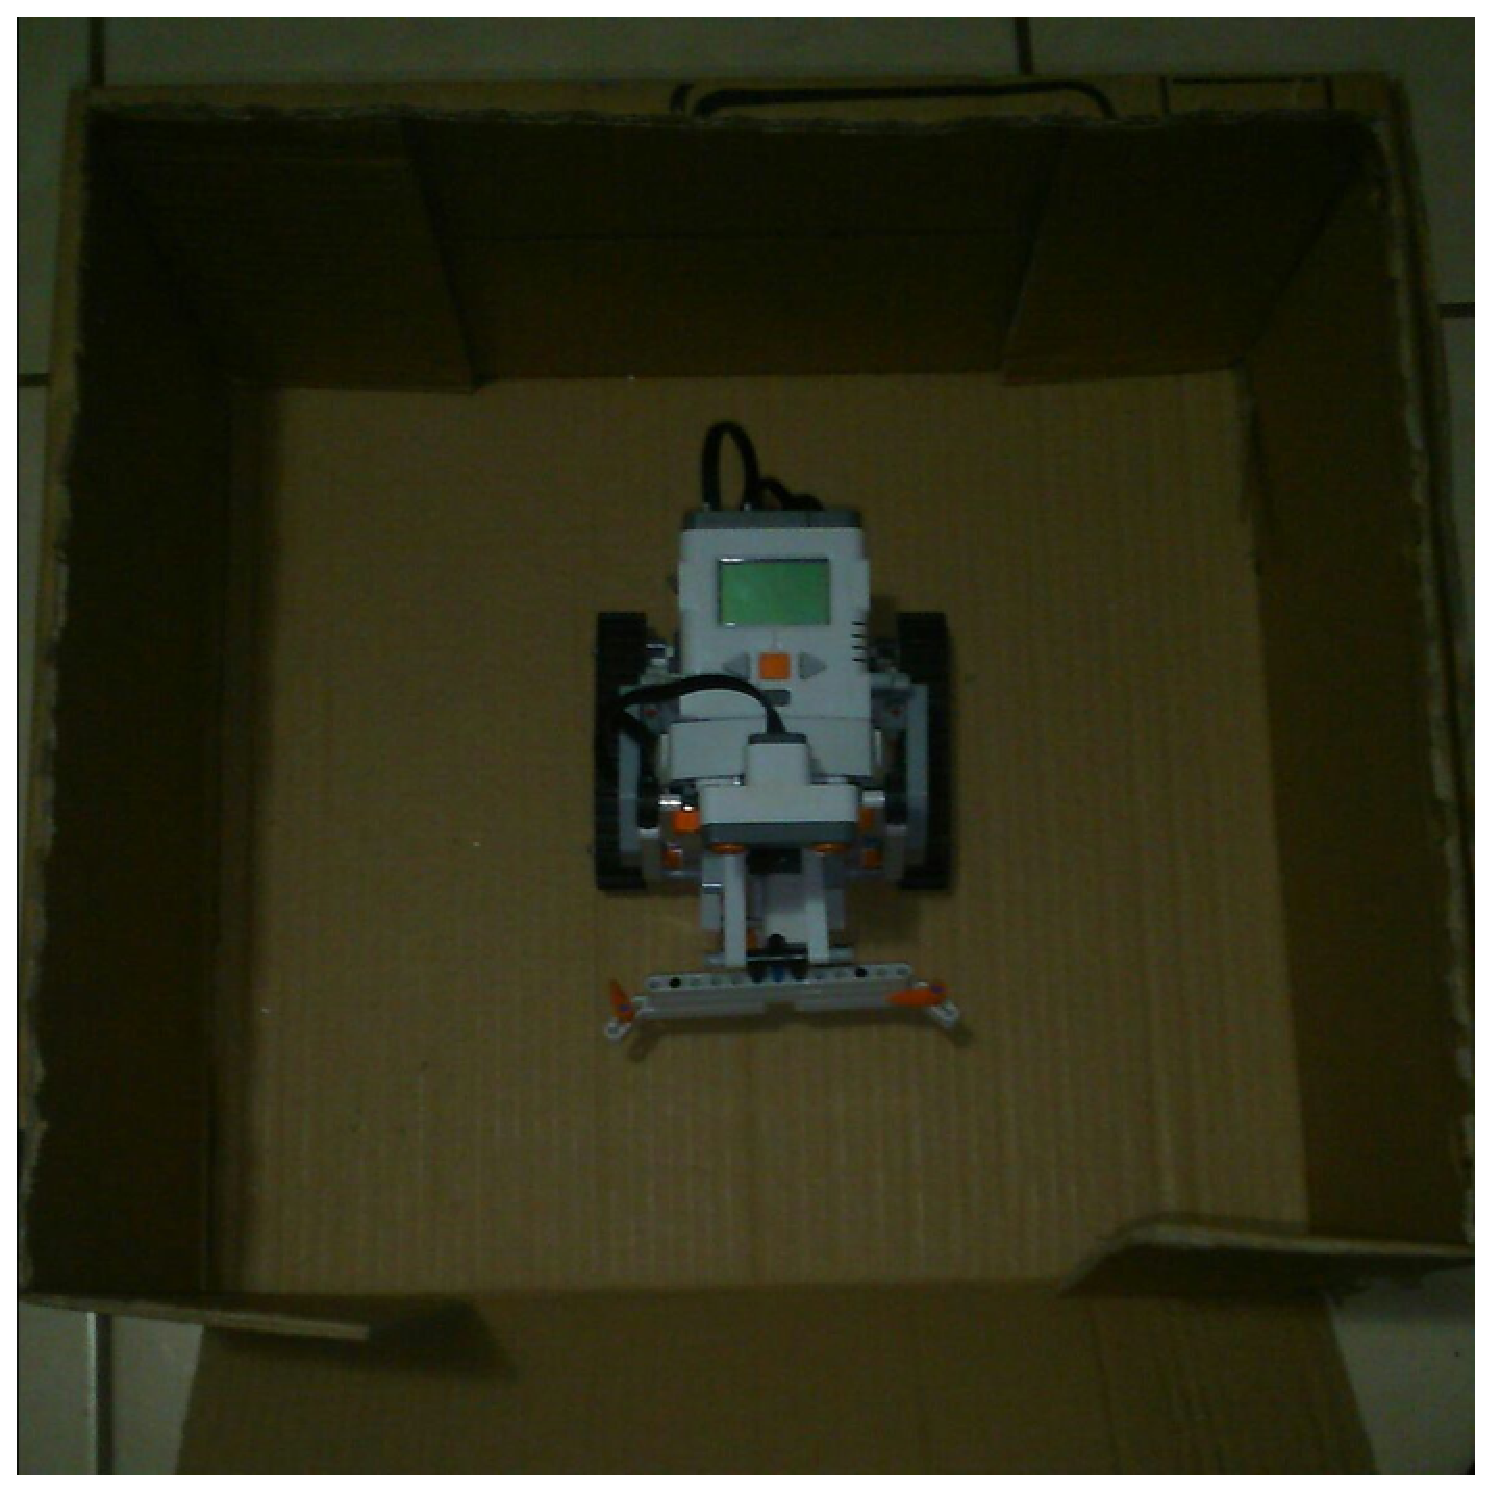
\includegraphics[scale=0.4]{figuras/ambienteConceito.eps}
			\label{img:ambienteProva}
			\caption{Ambiente prova de conceito}
		\end{figure}

		Com a realização da prova de conceito, ao implementar questões referentes ao posicionamento, direcionamento e localização do robô, diversas características foram identificadas e analisadas. Ao longo da seção \ref{sub:características_técnicas} estão apresentadas algumas destas características técnicas.

	% subsection planejamento_e_condução (end)

	\subsection{Características técnicas} % (fold)
	\label{sub:características_técnicas}
	
		Neste tópico serão apresentadas algumas das características importantes identificadas durante a realização da prova de conceito.

		\subsubsection{Seleção da linguagem e ambiente de desenvolvimento}

		Para realização desta prova de conceito, assim como o desenvolvimento de toda a solução proposta, ao longo do TCC\_2, optou-se pela utilização da linguagem Java. Esta escolha se deu não só devido à possibilidade, com mais facilidade, da integração desta solução com o \textit{framework} desenvolvido por \cite{tccRodrigo}, como também por todo o apoio técnico advindo da utilização da ferramenta \textit{leJOS NXJ}\footnote{http://www.lejos.org/nxj.php}.

		A ferramenta leJOS NXJ engloba, basicamente, uma máquina virtual Java (JVM) desenvolvida em C, sendo multiplataforma, ou seja, é portável para sistemas Linux, Windows e Macintosh \cite{legonxj}. O material de estudo sobre a ferramenta leJOS NXJ se encontra disponível em toda a \textit{web}, de maneira livre, e no livro \cite{legonxj}, que foi utilizado como fonte de informação durante o desenvolvimento.	

		O sistema operacional utilizado para realização desta prova de conceito foi o \textit{windows}, devido a sua facilidade de configuração da comunicação entre robô/PC, diferentemente do observado em sistemas Linux. O \textit{passo-a-passo} para instalação e configuração do ambiente utilizado para desenvolvimento se encontra em \cite[p. 6]{legonxj}.

		A seleção desta ferramenta é decorrente, além dos motivos apresentados anteriormente, da existência de uma \textit{API} que disponibiliza diversas funcionalidades referentes à navegação dos robôs. A \textit{API} do leJOS NXJ engloba desde funções referentes ao controle de motores, até o apoio a criação de mapas e sistemas complexos de navegação.

		Em paralelo à escolha da linguagem de programação, buscou-se identificar um ambiente de desenvolvimento que disponibilizasse ferramentas de apoio que facilitem o desenvolvimento da solução. Com este objetivo, optou-se pela utilização da \textit{IDE} Eclipse\footnote{https://eclipse.org/}, por possuir um \textit{plugin} da ferramenta leJOS NXJ, como apresenta \cite{legonxj}. O tutorial para instalação e configuração do ambiente utilizado se encontra em \cite[p. 14]{legonxj}.

	\subsubsection{Atuadores}

		Os atuadores, ou motores, contemplam a base da robótica móvel. Desse modo, o leJOS NXT disponibiliza diversas funcionalidades referentes ao controle destes atuadores. Um exemplo disso é a possibilidade de controlar a aceleração do motor, possibilitando um arranque com aceleração gradual, para minimizar as chances de derrapagem, por exemplo.

		Estas possibilidades de controle de rotação são devido a existência de \textit{encoders} óticos em cada motor, como apresenta \cite{legonxj}. Cada \textit{encoder} tem como objetivo registrar as rotações de cada eixo, possibilitando a navegação por odometria, como já foi explicado ao longo do trabalho.

		Para acessar os atuadores, o leJOS NXJ oferece, como principal fonte de acesso, a classe Motor, que possui três instâncias estáticas: \textit{Motor.A}, \textit{Motor.B} e \textit{Motor.C}. O livro \cite{legonxj} faz uma análise detalhada de todos os métodos presentes nesta classe, os quais são, principalmente, voltados à aceleração e velocidade de rotação dos eixos.

	\subsubsection{Sensores}

		Cada computador central do kit Mindstorms possui quatro portas para sensores, ou seja, a solução deste trabalho só pode envolver um máximo de quatro sensores, que fazem parte do kit Mindstorm. Para esta prova de conceito, foram utilizados os sensores de \textit{odometria}, a partir dos \textit{encoders} em cada atuador, um sensor ultrasônico, como sensor de distância e um sensor de toque.

		\begin{itemize}
			\item \textbf{Sensor de toque:}

				É o sensor mais básico do kit, que retorna um valor \textit{booleano} que indica se o sensor está pressionado ou não, a partir do botão laranja apresentado na figura \ref{img:sensorToque}.

				\begin{figure}[H]
					\centering
					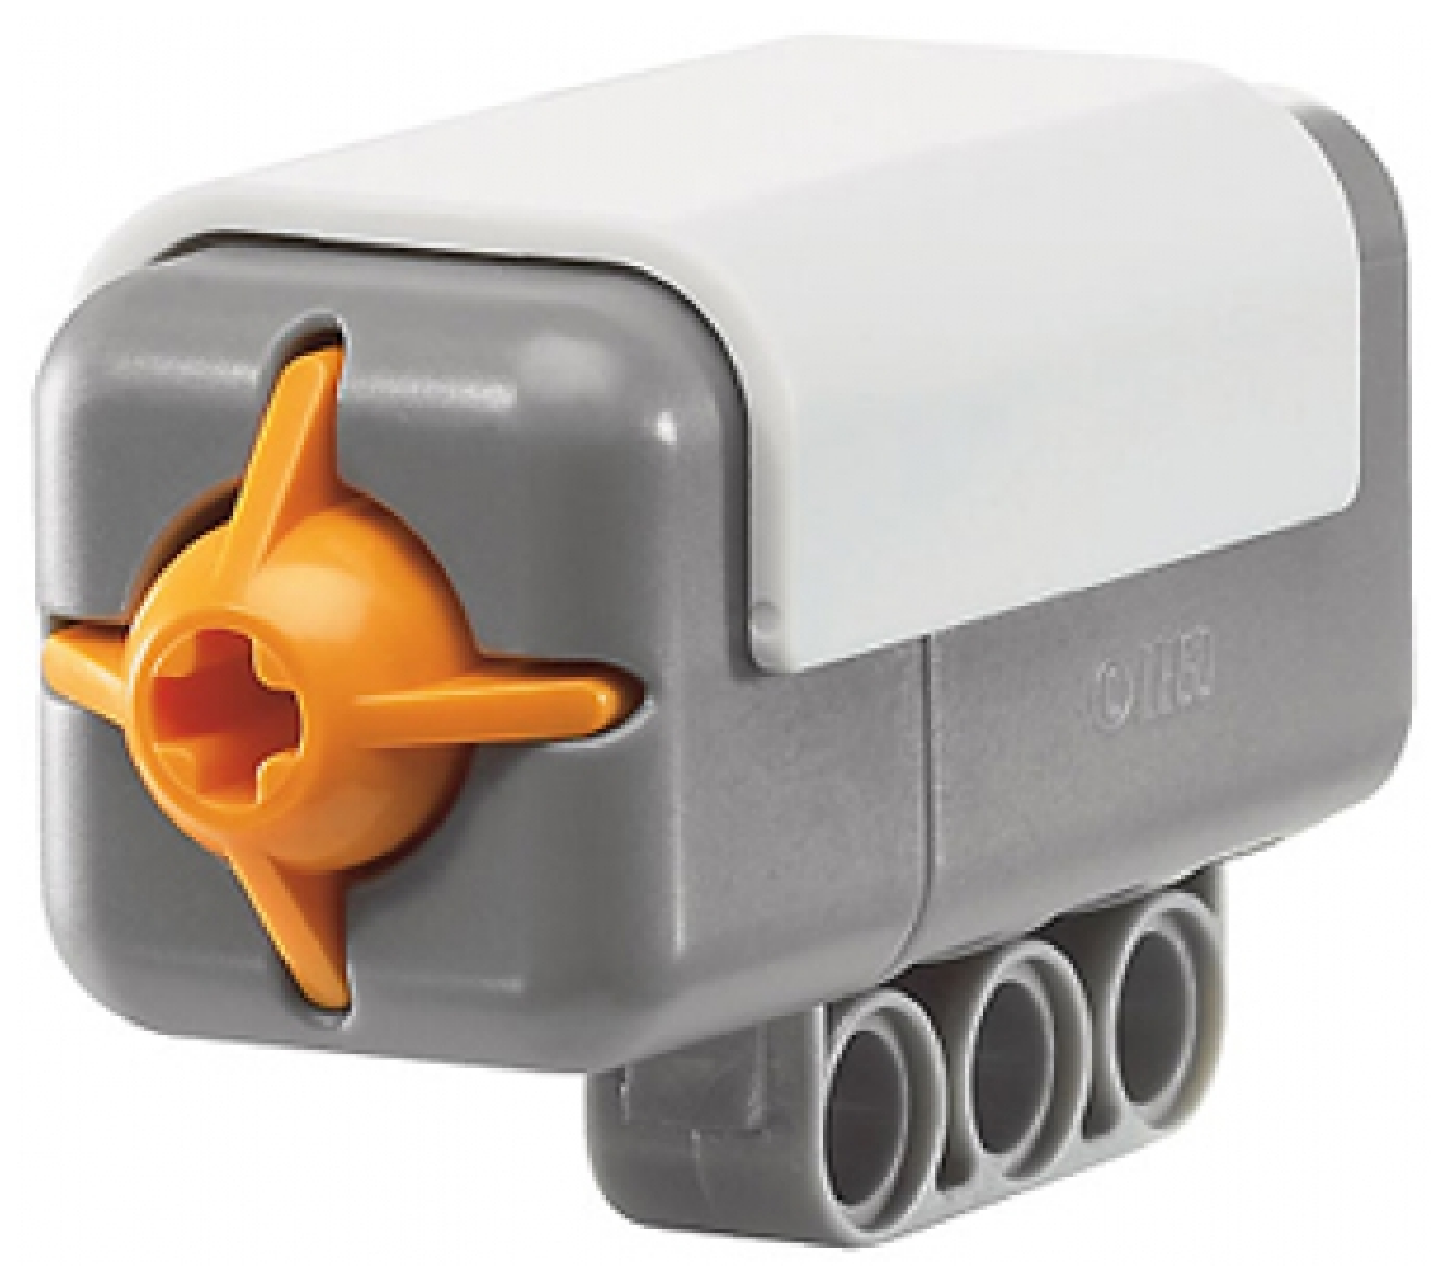
\includegraphics[scale=0.2]{figuras/sensorToque.eps}
					\caption{Sensor de toque.}
					\label{img:sensorToque}
				\end{figure}

				A classe \textit{TouchSensor}, que implementa a interface deste sensor, contém apenas um simples método: 

				\begin{lstlisting}
					boolean isPressed();
				\end{lstlisting}
			
			\item \textbf{Sensor ultrasônico:}

				Como apresenta a Figura \ref{img:ultrasonic}, o sensor ultrasônico lembra bastante um par de olhos, apesar de possuir muitas características em comum com um sensor de som, em vez de uma câmera, por exemplo. Isso se dá pela estratégia de funcionamento do sensor, o qual emite um sinal sonoro que reflete em obstáculos à frente, retornando ao sensor. A partir da análise do tempo percorrido pelo sinal sonoro, é possível estimar a distância do objeto analisado, em relação ao robô.

				\begin{figure}[H]
					\centering
					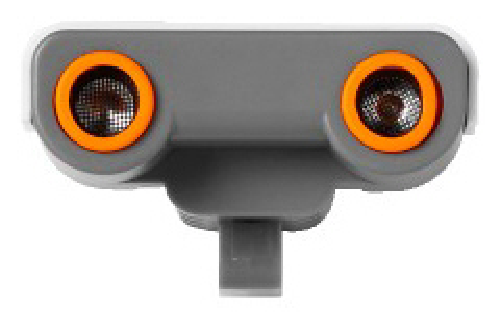
\includegraphics[scale=0.5]{figuras/ultrasonic.eps}
					\caption{Sensor ultrasônico.}
					\label{img:ultrasonic}
				\end{figure}

				Este sensor é capaz de identificar distâncias de até dois metros e meio, mais especificamente 255 centímetros. Porém, sua utilização em distâncias tão grandes não é recomendada por \cite{legonxj}, devido a grande margem de erro presentes em medições como esta. De acordo com \cite{legonxj}, este sensor possui, em distâncias de aproximadamente 180 centímetros, uma margem de erro de mais ou menos três centímetros (\textit{+/- 3}). Sua margem de erro é proporcional à distância entre robô e obstáculo.

				Outra característica importante do funcionamento deste sensor é a emissão de sinais no formato de cone, como apresenta a Figura \ref{img:cone2}\footnote{http://arcbotics.com/products/sparki/parts/ultrasonic-range-finder/}.


				\begin{figure}[H]
					\centering
					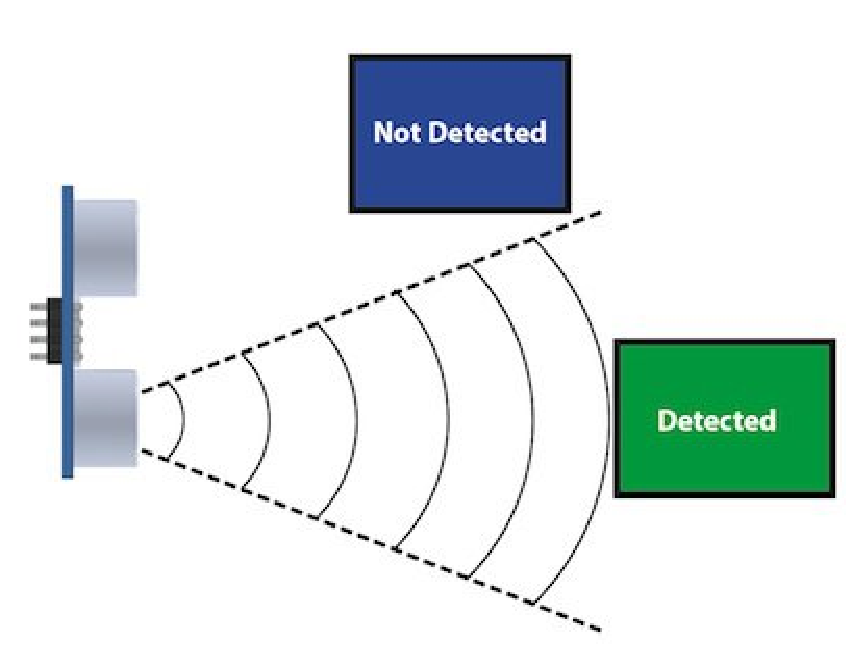
\includegraphics[scale=0.7]{figuras/cone2.eps}
					\caption{Emissão do sinal ultrasônico.}
					\label{img:cone2}
				\end{figure}

				O cone formado pela emissão do sinal segue uma angulação de 30º, ou seja, em uma distância de 180 centímetros, o cone possui um diâmetro de 90 centímetros. Desse modo, deve-se levar em consideração a incapacidade de identificar pequenas irregularidades em obstáculos, como fendas e buracos.

				Durante o desenvolvimento da prova de conceito, observou-se com mais precisão a característica descrita acima, levando à alteração da proposta do trabalho, em relação ao ambiente utilizado. Inicialmente, o ambiente proposto se baseava no tapete de missões \textit{Nature's Fury}, utilizado como um dos desafios do torneio \textit{First Lego League}\footnote{http://www.firstlegoleague.org/}. Um exemplo deste ambiente pode ser visualizado na Figura \ref{img:tapete}.

				\begin{figure}[H]
					\centering
					\includegraphics[scale=0.4]{figuras/tapete.eps}
					\caption[Ambiente proposto inicialmente]{Ambiente utilizado.}
					\label{img:tapete}
				\end{figure}

				Os problemas referentes aos cantos, buracos e fendas encontrados durante a realização da prova de conceito mostraram o grande impacto desta característica do sonar no mapeamento de ambientes pequenos, como o utilizado. Desse modo, optou-se por modificar o ambiente a ser utilizado durante a segunda etapa deste trabalho. O ambiente será baseado em cômodos reais, como quartos, salas ou escritórios. O critério inicial para utilização do ambiente é referente a área de navegação disponivel, devendo ser de, pelo menos, 2 metros quadrados.

		\end{itemize}

		\subsubsection{Computador central NXT (Brick)} % (fold)
		\label{sub:brick}

			O robô utilizado durante esta prova de conceito e durante o desenvolvimento da solução proposta, é da família Mindstorm NXT, da Lego. O computador central, de acordo com \cite{legonxj}, possui uma área de 7,2 x 11,2 centímetros, com um processador \textit{Atmel 32-bit ARM} de 48 MHz de frequência, memória RAM de 64 KB e 256 KB de memória \textit{flash}.

			Estas limitações de memória e processamento foram contornadas a partir da utilização da arquitetura de processamento remoto, como foi definido na seção \ref{sec:adaptação_e_implementação}, já como um resultado da revisão sistemática apresentada na seção \ref{sec:revisão_sistemática}.
		
		% subsection  (end)



	% subsection características_técnicas (end)
% section desenvolvimento_prático (end)

\section{Considerações parciais} % (fold)
\label{sec:consideracoes}
	
	Neste capítulo foram apresentados os resultados obtidos durante a realização da primeira estapa deste trabalho (TCC\_1). Como principal resultado, se encontra a revisão sistemática realizada, que possibilitou a ampliação dos conhecimentos relacionados a área de atuação, assim como de detalhes importantes da escrita científica, até o momento desconhecidos pelo autor.

	A identificação das técnicas e soluções do problema de SLAM com a revisão sistemática apresentou como resultado padrões de soluções em diversos contexto. Como um exemplo destes padrões, temos a utilização da arquitetura de processamento remoto na maioria das pesquisas obtidas durante a revisão. Desse modo, observou-se a inquestionável vantagem da utilização desta arquitetura, o que definiu sua utilização durante a realização deste trabalho.

	Outro resultado bastante importante da revisão sistemática é a confirmação dos filtros mais utilizados pela acamedia de robótica como sendo o filtro de Kalman e o filtro de partículas. A escolha do filtro a ser utilizado neste trabalho ainda não foi realizada, pois necessita de maiores conhecimentos sobre a implementação dos mesmos.

	Já os resultados obtidos em relação a parte prática desta pesquisa, estão definidos como uma série de características identificadas durante a implementação da prova de conceito. Sua realização possibilitou a confirmação da viabilidade da utilização da arquitetura de processamento remoto, assim como a definição da linguagem a ser utilizada, os sensores e a montagem do robô a ser utilizada ao longo de todo o trabalho.

	Durante a segunda etapa do trabalho, pretende-se evoluir a prova de conceito apresentada durante esta primeira etapa, buscando solucionar, de maneira simplificada, o problema de SLAM. A partir dos ciclos de desenvolvimento, serão realizadas análises referentes às peculiaridades encontradas ao implementar técnicas de auto-localização em robôs simples, assim como o impacto desta implementação em um contexto educacional.

	A escolha do filtro probabilístico que será utilizado será feita durante a realização da segunda etapa do trabalho, a partir de análises da exigência computacional e complexidade de implementação. 

% section section_name (end)